\documentclass[11pt, a4paper]{article}


%%%% Encodings

\usepackage[utf8]{inputenc} % encoding
\usepackage[english]{babel} % use special characters and also translates some elements within the document.

%%%% Misc

\usepackage{hyperref}       % Hyperlinks \url{url} or \href{url}{name}
\usepackage{parskip}        % \par starts on left (not idented)
\usepackage{tocbibind}      % Adds the bibliography to the table of contents (automatically)

% \usepackage[document]{ragged2e}  % Left-aligned (whole document)
% \begin{...} ... \end{...}   flushleft, flushright, center

%%%% Abstract

\usepackage{abstract}       % Abstract

% http://www.ctex.org/documents/packages/special/abstract.pdf
\renewcommand{\absnamepos}{flushleft} % \begin{abstract} \noindent ... \end{abstract}
\setlength{\absleftindent}{0pt}
\setlength{\absrightindent}{0pt}

%%%% Graphics

\usepackage{graphicx}
\graphicspath{{./figures/}} % directory to look up for graphics

% \begin{figure}[h]
%   \centering
%   \includegraphics[scale=0.5]{cat}  % [width=\textwidth, height=4cm],
%   \caption{Example of a cat}
%   \label{fig:cat}
% \end{figure}

%%%% Math

\usepackage{amsmath}        % Math
\usepackage{amssymb}        % New symbols http://milde.users.sourceforge.net/LUCR/Math/mathpackages/amssymb-symbols.pdf
\usepackage{bm}             % $\bm{D + C}$

\usepackage{amsthm} % Math, \newtheorem, \proof, etc
% \begin{theorem}\label{t:label}  ...  \end{theorem}
% \begin{proof} ... \end{proof}
\theoremstyle{plain} % default
\newtheorem{theorem}{Theorem}[section]
\newtheorem{corollary}{Corollary}[theorem]  % Numering depends on the current section (instead of global)
\newtheorem{lemma}[theorem]{Lemma} % Shares numeration with theorem.
\theoremstyle{definition}
\newtheorem{definition}{Definition}[section]
\theoremstyle{remark}
\newtheorem*{remark}{Remark}

% Defines a new environment to write your or claim - proof
\newenvironment{claim}[1]{\par\noindent\underline{Claim:}\space#1}{}
\newenvironment{claimproof}[1]{\par\noindent\underline{Proof:}\space#1}{\hfill $\blacksquare$}

%%%% Code/Pseudo-code

\usepackage{minted} % Code listing
% \mint{html}|<h2>Something <b>here</b></h2>|
% \inputminted{octave}{BitXorMatrix.m}

%\begin{listing}[H]
  %\begin{minted}[xleftmargin=20pt,linenos,bgcolor=codegray]{haskell}
  %\end{minted}
  %\caption{Example of a listing.}
  %\label{lst:example} % You can reference it by \ref{lst:example}
%\end{listing}

\newcommand{\code}[1]{\texttt{#1}} % Define \code{foo.hs} environment

\usepackage[vlined,ruled]{algorithm2e} % pseudo-code http://tug.ctan.org/macros/latex/contrib/algorithm2e/doc/algorithm2e.pdf

%%%% Colors

\usepackage{xcolor}         % Colours \definecolor, \color{codegray}
\definecolor{codegray}{rgb}{0.9, 0.9, 0.9}
% \color{codegray} ... ...
% \textcolor{red}{easily}

%%%% Math

%\makeglossaries % before entries

%\newglossaryentry{latex}{
    %name=latex,
    %description={Is a mark up language specially suited
    %for scientific documents}
%}

% Referene to a glossary \gls{latex}
% Print glossaries \printglossaries

\usepackage[acronym]{glossaries} %

% \acrshort{name}
% \acrfull{name}
% \newacronym{foo}{arcshort}{acrfull}

\usepackage{enumitem} % \begin{enumerate}[label=(\alph*)]



\renewcommand{\thesection}{\Alph{section}}
\renewcommand{\thesubsection}{\thesection.\arabic{subsection}}

\usepackage[
backend=biber,
style=alphabetic,
sorting=ynt
]{biblatex}

\addbibresource{bibliography.bib}

\usepackage{fancyhdr}
\usepackage{listings}
\usepackage{graphicx}
\usepackage{url}
\pagestyle{fancy}
\fancyhf{}
\rhead{ML}
\lhead{FIB - UPC}
\rfoot{Page \thepage}

\title{%
  \vspace{-10ex}
  ML: Project \\
  \large{MIRI}
}
\author{%
  Arnau Abella \\
  Antoni Casas \\
  \\
  \large{Universitat Polit\`ecnica de Catalunya}
}
\date{\today}

%%%%%%%%%%%%%%%%%%%%%%%%%%%%%%%%%%%%%%%%%%%%%%%%%%%%%%%%%

\begin{document}
\maketitle

\section{Project description}

Strokes are an unexpected killer and hard to predict, being the second leading cause of death globally. Therefore, the detection of segments of the population at risk could enhance the ability of hospitals and other medical teams to offer early treatments and screenings to reduce this risk.

A stroke occurs when the blood supply to part of your brain is interrupted or reduced, preventing brain tissue from getting oxygen and nutrients. Brain cells begin to die in minutes. A stroke is a medical emergency, and prompt treatment is crucial. Early action can reduce brain damage and other complications. Effective treatments can also help prevent disability from stroke.

For this purpose, we make use of the stroke prediction dataset, a dataset composed of 11 variables, and 1 variable to predict with 5110 observations. The variables present are:

\begin{table}[H]
\begin{tabular}{ll}
Gender                & Categorical \\
Age                   & Numerical   \\
Hypertension          & Binary      \\
Heart Disease         & Binary      \\
Ever Married          & Binary      \\
Work Type             & Categorical \\
Residence Type        & Categorical \\
Average Glucose Level & Numerical   \\
BMI                   & Numerical   \\
Smoking Status        & Categorical \\
Stroke                & Binary     
\end{tabular}
\end{table}

\section{Previous work}

Being a Kaggle dataset, it has some previous analysis, though most of the works seem to ignore the unbalacedness of the dataset and jump straight to achieving a 95\% accuracy, on a 95 / 5 unbalanced dataset, which is a less than optimal approach. Following that, we ignore any work that didn't take into account the unbalancedness of the data, some models reaching to the point where there's barely any single value in the minority class, like in  \cite{mariahchristy_2021}. 

Even worse, those who took into account the unbalancedness of the data and applied a resampling technique, generated data leakage by resampling their test set too, leading to wrong measures of generalization, as seen on \cite{paytonfisher_2021}.

Therefore, on our work we will focus on not generating data leakage and taking into account the unbalancedness of the data to achieve a better model with a more appropriate approximation of the generalization error.


\section{Data exploration}

First we begin by looking at the distribution of our categorical variables, which as seen on figure \ref{fig:categoricalVariables}, with the exception of two categories, one on Gender and one on Work Type, are well represented, having a sufficient amount of samples

\begin{figure}[H]
    \centering
    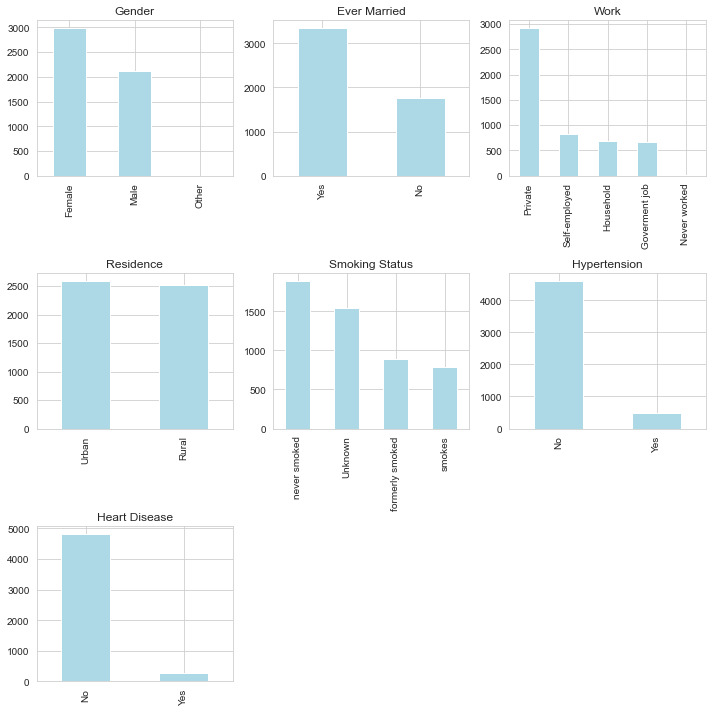
\includegraphics[width=0.8\textwidth]{images/catDest.jpg}
    \caption{Categorical Variable Distribution}
    \label{fig:categoricalVariables}
\end{figure}

Our numerical variables seem to follow a mixture of Gaussians, as seen on Figure \ref{fig:KDE}. Comparing the distribution of those observations with stroke and those without stroke, we can see that there seems to be a difference, but it doesn't seem too pronounced. We can see that there seem to be outliers in both age and BMI, however, we do not want to exclude edge cases of age, as they seem to be important based on their distribution. We will, however, remove those BMI lower than 15 and higher than 60, and replace them by either 15 or 60, this is because those values are extreme outliers in real life \cite{BMI}.

Looking at the kernel density in Figure \ref{fig:KDE} estimate but in a pair-wise manner, we can see that stroke only occupies a small section of the planes, but seems to overlap with non-strokes, which seems to indicate that our model will have to focus on those boundaries, since overfitting seems likely.

\begin{figure}[H]
    \centering
    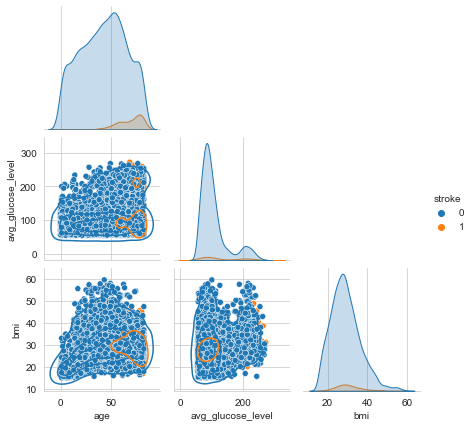
\includegraphics[width=0.8\textwidth]{images/KDE.png}
    \caption{Kernel Density Estimate}
    \label{fig:KDE}
\end{figure}

Observing the variable correlations, we see some interesting relations, like marriage and age being highly correlated, but we do not observe a highly meaningful correlation between stroke and any variable, the closest being age. However, these low correlations also mean that colinearity won't be an issue.

\begin{figure}[H]
    \centering
    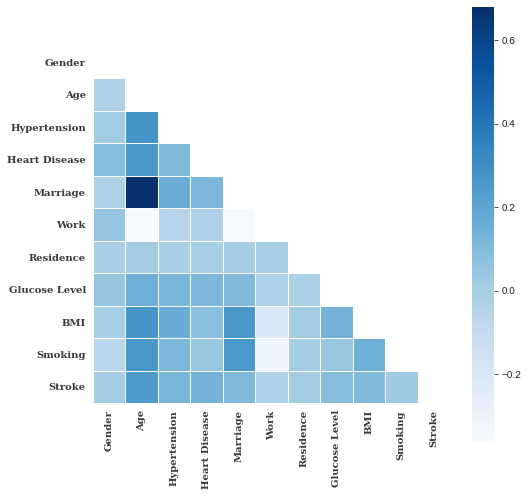
\includegraphics[width=0.8\textwidth]{images/Correlation.png}
    \caption{Correlation Map}
    \label{fig:Correlation}
\end{figure}


To help us get a better understanding of our data, we decide to perform MCA to get a better idea of how the variables interact with each other, to do this, first we discretize our numeric variables using expert knowledge, and then perform MCA. As can be seen on the plot obtained by MCA on figure \ref{fig:mca}, as we can see, our variables are ordered on this new feature space along the x-axis, so we can observe that these relations, even on discretized data, which has lost information respective to its true numeric data. This lets us know that there seems to be a relation between those "unhealthy" categories, on the negative x-axis, and the "healthy" categories, on the positive x-axis. 

\begin{figure}[H]
    \centering
    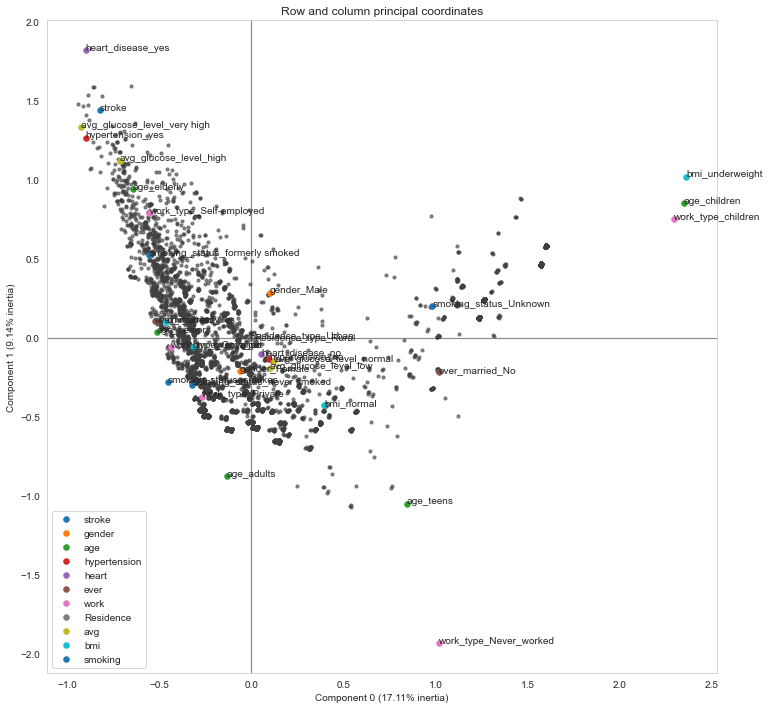
\includegraphics[width=0.8\textwidth]{images/MCA.png}
    \caption{MCA visualization}
    \label{fig:mca}
\end{figure}


The number of missing values is low, only present on the BMI variable, and being 258 missing values out of 5110, as seen on Figure \ref{fig:missingValues}, for this purpose, we decide to keep these observations and follow a method of data imputation, a decision tree based on age, marriage and hypertension.

\begin{figure}[H]
    \centering
    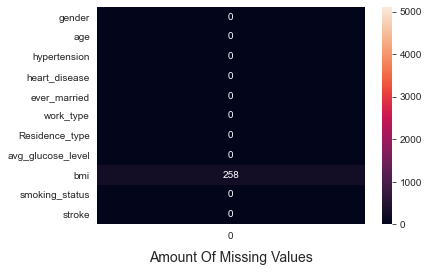
\includegraphics[width=0.8\textwidth]{images/MissingValues.png}
    \caption{Missing Values}
    \label{fig:missingValues}
\end{figure}


\section{Preprocessing}


To prepare our dataset for classification, we perform one-hot encoding on our categorical variables, so as to obtain a numerical representation, since the number of factors we have in each categorical variable isn't too large, we decided not to remove categories below a certain frequency.

Standardization of numerical values was performed so as to make the numerical variables compatible with all methods.


Finally taking into account the distribution of this dataset on our variable to predict, stroke, which is severely imbalanced, with a 4.9\% of positive cases and 95.1\% of negative cases we choose SMOTE with Tomek links, which performs a resampling using SMOTE, and then undersampling using Tomek links, that is, if the nearest neighbor of a majority class sample is of the minority class, remove the majority class sample. This will lower the imbalance in training so as to reduce the overfitting that would appear from only having 5\% of one class.

\begin{figure}[H]
    \centering
    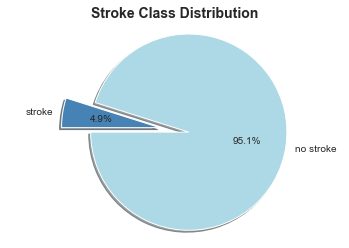
\includegraphics[width=0.8\textwidth]{images/Stroke.png}
    \caption{Stroke distribution}
    \label{fig:stroke}
\end{figure}

After applying SMOTE and undersampling with Tomek links, our train set has 2900 examples of the minority class and 2900 examples of the majority class, achieving a perfectly balanced training set. 


\section{Modelling methods considered}

We considered as model candidates:

Linear Models: Logistic Regression \\
Discriminant Analysis: LDA and QDA \\
Clustering: k-NN \\
Support Vector Machines: SVC \\
Trees: CART \\
Ensemble Methods: Random Forest, AdaBoost, GradientBoostingClassifier, Voting Classifier \\
Bayes Classifier: Naive Bayes \\
Neural Networks: MLP \\

Our candidates are varied, but we know from the outset most will perform extremely poorly due to the nature of the data, like Naive Bayes, even then, we use them to get a better insight into our data, as it helps us understand how to avoid overfitting in the minority class via letting us see which type of approach performs better.

\subsection{Validation method}

The validation method followed is as follows. 

We separate our data into test and train sets, with 20\% going to test and 80\% going to train and validation, with a further 25\% of train going to a validation set. Our test and validation data is completely separate from our train data, where even our data imputation model is built entirely upon our train data. 

For our model selection and hyperparameter tuning, we use cross-validation over our train set with 5 folds, and we evaluate the model on the validation set, which does not have data imputed by SMOTE nor has been undersampled with Tomek links, giving us a better overview of how well will it generalize. 

Finally, after our model is chosen, we validate the chosen model over the test set to get an overview of its true generalization ability.


\begin{figure}[H]
    \centering
    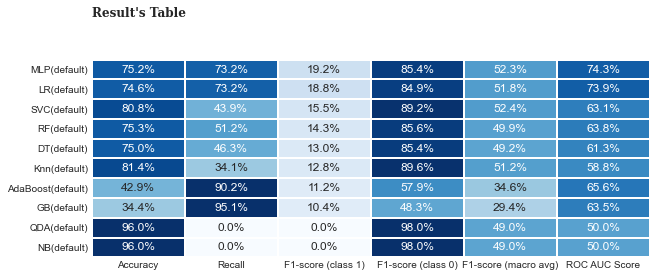
\includegraphics[width=\textwidth]{images/Accuracies.png}
    \caption{Stroke distribution}
    \label{fig:accuracies}
\end{figure}

All our models, with no hyperparameter tuning, perform extremely poorly on positive examples of Stroke, which is what we want to focus on, as a false negative of a Stroke is much more dangerous than a false positive, as one might involve death. Following this, our initial chosen models are:

Multi-layer perceptron: 19.2\% F1-score on minority class \\
Logistic Regression: 18.8\% F1-score on minority class \\
Random Forest:  14.3\% F1-score on minority class \\
Decision Trees: 13.0\% F1-score on minority class \\
Voting Classifier: Ensemble of our 2 best models\\

The F1 scores mentioned are as seen on Figure \ref{fig:accuracies}. SVM wasn't taken due to being outperformed by linear regression, which might indicate that any kernel might add too much complexity and generate overfitting.

\subsection{Model tuning}


\subsubsection{Decision Tree}

For optimization we considered the following parameters: minimal amount of samples for a leaf, minimal amount of samples for a split, maximum amount of features, maximum tree depth, criterion.

The optimized model was one with entropy as its criterion, no maximum depth, automatic maximum feature selection, 1 sample needed for a leaf, and 5 samples needed for a split. Resulting in the best model with the results as seen in Figure \ref{fig:confMatDecTree}.  The best model leaves a lot to be desired, but at least achieves 44\% of true positives in the minority class, this is further observed in the poor RoC curve seen in Figure \ref{fig:RoCDT}, which is too close to the diagonal.

Looking at the feature importance obtained, age dominates in importance, with glucose level and bmi far behind, with importance quickly dropping off. 

\begin{table}[H]
\begin{tabular}{|l|l|}
\hline
age                           & 0.434334 \\ \hline
avg\_glucose\_level           & 0.131974 \\ \hline
bmi                           & 0.105249 \\ \hline
Residence\_type\_Urban        & 0.080001 \\ \hline
gender\_Male                  & 0.053817 \\ \hline
work\_type\_Private           & 0.035850 \\ \hline
ever\_married\_Yes            & 0.026716 \\ \hline
smoking\_status\_smokes       & 0.024044 \\ \hline
smoking\_status\_never smoked & 0.021232 \\ \hline
work\_type\_Self-employed     & 0.020924 \\ \hline
\end{tabular}
\end{table}

%Have to fix the confusion matrix size, this is an abomination


\begin{figure}[H]
\minipage{0.5\textwidth}
    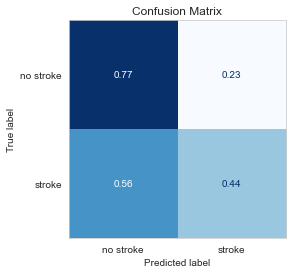
\includegraphics[width=\textwidth]{images/confMatDecTree.png}
    \caption{Confusion Matrix D.T.}
    \label{fig:confMatDecTree}
\endminipage\hfill
\minipage{0.5\textwidth}
    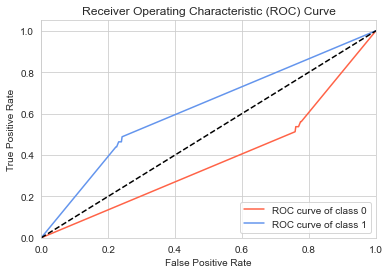
\includegraphics[width=\textwidth]{images/rocDT.png}
    \caption{RoC Curve D.T.}
    \label{fig:RoCDT}
\endminipage\hfill
\end{figure}


\subsubsection{Random Forest}

For optimization we considered the following parameters: minimal amount of samples for a leaf, minimal amount of samples for a split, maximum tree depth, and number of estimators and class weight.

The optimized model was one with, 4 samples needed for a leaf, 4 samples needed for a split, 100 estimator, maximum tree depth of 100 and balanced class weight. Resulting in the best model with the results as seen in Figure \ref{fig:randForConfMat}.  The best model leaves a lot to be desired, but at least achieves 59\% of true positives in the minority class, which is a straight improvement from the Decision Tree, as should be expected from a Random Forest classifier. The RoC curve also seems to distance itself from the diagonal, while not a lot, a definite improvement over the decision tree, as seen on Figure \ref{fig:RoCRF}.


%Have to fix the confusion matrix size, this is an abomination

\begin{figure}[H]
\minipage{0.5\textwidth}
    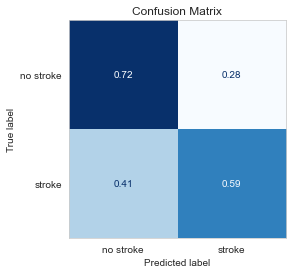
\includegraphics[width=\textwidth]{images/randForConfMat.png}
    \caption{Confusion Matrix R.F.}
    \label{fig:randForConfMat}
\endminipage\hfill
\minipage{0.5\textwidth}
    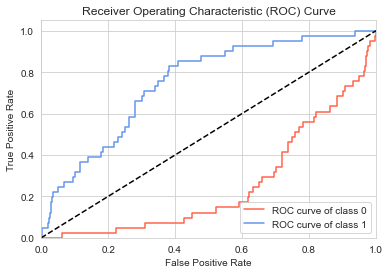
\includegraphics[width=\textwidth]{images/rocRF.png}
    \caption{RoC Curve R.F.}
    \label{fig:RoCRF}
\endminipage\hfill
\end{figure}

\subsubsection{Logistic Regression}


For optimization we considered the following parameters: C (regularization parameter), maximum number of iterations and penalty, only considering $L_1$ and $L_2$ loss.

The optimized model was one C equal to 0.01, with 100 iterations and L2 loss. Resulting in the best model with the results as seen in Figure \ref{fig:logRegConfMat}.  The best model once again leaves a lot to be desired, but at least achieves 76\% of true positives in the minority class, which is a straight improvement from the Random Forest, it seems our issue is overfitting, and logistic regression, being robust to overfitting, is performing the best. The RoC graph seems to corroborate this conclusion, as the RoC curve separates nicely from the diagonal, as seen on Figure \ref{fig:RoCLog}

%Have to fix the confusion matrix size, this is an abomination

\begin{figure}[H]
\minipage{0.5\textwidth}
    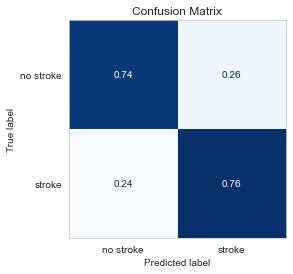
\includegraphics[width=\textwidth]{images/logRegConfMat.png}
    \caption{Confusion Matrix Logistic Regression $L_2$}
    \label{fig:logRegConfMat}
\endminipage\hfill
\minipage{0.5\textwidth}
    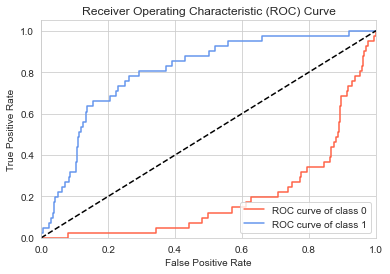
\includegraphics[width=\textwidth]{images/rocLog.png}
    \caption{RoC Curve}
    \label{fig:RoCLog}
\endminipage\hfill
\end{figure}


\subsubsection{Multi-layer perceptron}

For our MLP parameters, we only considered different architectures and the alpha value. With our winning architecture being two layers of 8 perceptrons with an alpha value of 1. The best model is severely worse than the one we obtained with logistic regression, seemingly reinforcing our guess that the problem is entirely within overfitting, as seen in Figure \ref{fig:mlpConfMat}. The RoC curve has also worsened considerably in comparison to the logistic regression, being much closer to the diagonal, as seen in Figure \ref{fig:RoCMLP}.

%Have to fix the confusion matrix size, this is an abomination

\begin{figure}[H]
\minipage{0.5\textwidth}
    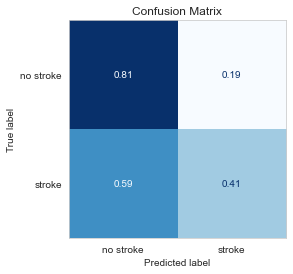
\includegraphics[width=\textwidth]{images/mlpConfMat.png}
    \caption{Confusion Matrix MLP}
    \label{fig:mlpConfMat}
\endminipage\hfill
\minipage{0.5\textwidth}
    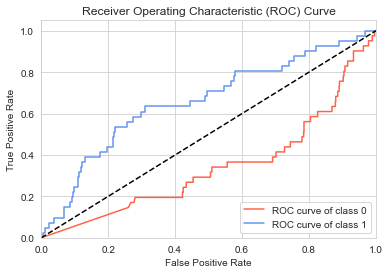
\includegraphics[width=\textwidth]{images/rocMLP.png}
    \caption{RoC Curve}
    \label{fig:RoCMLP}
\endminipage\hfill
\end{figure}

\subsubsection{Voting Classifier}

For our voting classifier, we considered using our two best models, as obtained in our logistic regression and random forest hyperparameter tuning sections, and tested whether to use soft or hard voting, with soft voting giving the best results of the voting classifier, as seen on Figure \ref{fig:votSoftMat}. Being made of both the linear regression and random forest models, its RoC is rather good, being rather separated from the diagonal, as seen in Figure \ref{fig:RoCVoting}.

%Have to fix the confusion matrix size, this is an abomination

\begin{figure}[H]
\minipage{0.5\textwidth}
    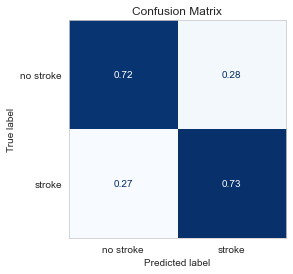
\includegraphics[width=\textwidth]{images/softConfMat.png}
    \caption{Confusion Matrix Soft Voting}
    \label{fig:votSoftMat}
\endminipage\hfill
\minipage{0.5\textwidth}
    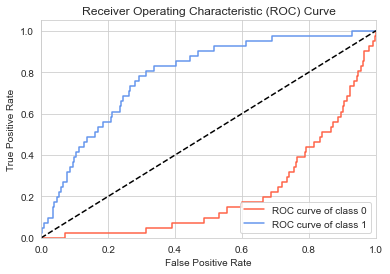
\includegraphics[width=\textwidth]{images/rocVoting.png}
    \caption{RoC Curve}
    \label{fig:RoCVoting}
\endminipage\hfill
\end{figure}


\section{Final model chosen}

Looking at what models are doing better and which parameters are improving results, it seems that the issue is severe overfitting due to the data imbalance, which means that our best model should be the most robust model against overfitting, which, amongst the three we chose, is the Logistic Regression with L2 loss, which also leads to the best results.


\begin{figure}[H]
\minipage{0.5\textwidth}
    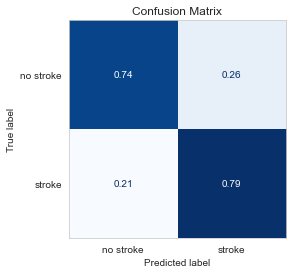
\includegraphics[width=\textwidth]{images/LogRedResult.png}
    \caption{Confusion Matrix Test Linear Regression}
    \label{fig:logRegFinal}
\endminipage\hfill
\minipage{0.5\textwidth}
    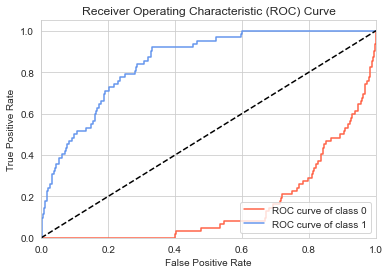
\includegraphics[width=\textwidth]{images/rocFinak.png}
    \caption{RoC Curve}
    \label{fig:RoCCurve}
\endminipage\hfill
\end{figure}

Even with our optimized model, the results are somewhat poor, they are, however, better than our metrics obtained in the validation set, even if only very slightly, since, as seen on Figure \ref{fig:logRegFinal}, where the true positives of the minority class raise to 79\%. This means that it seems to be an accurate representation of its generalization capability.

 We can also see on the RoC graph of Figure \ref{fig:RoCCurve} that this model has an interesting quirk, and that is that we can achieve a true positive rate of 100\% on the minority class if we also have a false positive rate of 60\% in the minority class, which means we can effectively never miss a possible stroke if we are willing to also deal with all the false positives, which might be a possibility.


\section{Conclusions}

Out of all our models, the ones most robust to overfitting were the only ones who managed to perform well on the minority class, we believe this to be a case of a lack of data, since certain spaces of the hyperplane are left either unpopulated or with so little population that boundaries cannot be established properly, leading to overfitting and poor generalization.

Our best model was the logistic regression with L2 loss, a simple linear method, but extremely hard to overfit, with an interesting RoC curve, which could be exploited to obtain the best balance between false positives and true positives, since the focus is on achieving the highest number of true positives on the minority class, since a misdiagnosis can be fatal.

We can also see that of all the variables, those with the highest effect on stroke are, first of all and by far, age, then far behind average glucose level and bmi, with the rest of variables trailing behind. These relations might help understand strokes better.



\section{Future work}

The data seems too poor to be able to create a good model for the minority class, however, it might be possible that there exists a transformation where, in the new space, the data is good enough to generalize with the current data.

Ignoring such event, the only possible work is expanding the data, be it via new variables recorded, or by adding more samples, as otherwise, this dataset seems too poor, as only methods robust enough against overfitting obtained the best results.

\section{Bibliography}
\printbibliography

\end{document}

